\makeatletter
\def\input@path{{poster_template/poster}}
\makeatother

\documentclass[final]{beamer}

\usepackage[scale=1.24]{beamerposter}

\usetheme{confposter}

\setbeamercolor{block title}{fg=ngreen,bg=white}
\setbeamercolor{block body}{fg=black,bg=white}
\setbeamercolor{block alerted title}{fg=white,bg=ngreen!70} 
\setbeamercolor{block alerted body}{fg=black,bg=ngreen!10}

\newlength{\sepwid}
\newlength{\onecolwid}
\newlength{\twocolwid}
\newlength{\threecolwid}
\setlength{\paperwidth}{48in}
\setlength{\paperheight}{36in}
\setlength{\sepwid}{0.024\paperwidth}
\setlength{\onecolwid}{0.22\paperwidth}
\setlength{\twocolwid}{0.464\paperwidth}
\setlength{\threecolwid}{0.708\paperwidth}
\setlength{\topmargin}{-0.5in}

\usepackage{graphicx}
\usepackage{booktabs}
\usepackage{xcolor}
\usepackage{amsmath}
\usepackage{url}

\definecolor{ngreen}{RGB}{34,139,34}
\definecolor{dblue}{RGB}{0,0,139}
\definecolor{titletextcolor}{RGB}{50,50,50}
\definecolor{secondarycolor}{RGB}{100,100,100}
\definecolor{primarycolor}{RGB}{0,0,0}
\setbeamercolor{cboxb}{fg=black,bg=ngreen}  


\DeclareMathOperator*{\argmax}{argmax}
\DeclareMathOperator*{\argmin}{argmin}

\newcommand{\longeqsize}{\fontsize{20.5}{26}\selectfont}
%----------------------------------------------------------------------------------------
% META INFORMATION
%----------------------------------------------------------------------------------------

\title[Word Translation Without Parallel Data]{\textcolor{ngreen}{Word Translation Without Parallel Data (2018)}}
\author[ ]{\textcolor{secondarycolor}{A. Conneau, G. Lample, M. Ranzato, L. Denoyer, H. Jégou\\Poster by: A. Puigdemont Monllor, J. Čieško}}
\institute[FI MU]{\textcolor{secondarycolor}{PA164: Machine Learning and NLP, Faculty of Informatics, Masaryk University, November 11, 2024}}
\date{\textcolor{primarycolor}{November 11, 2024}}

%----------------------------------------------------------------------------------------

\begin{document}

\addtobeamertemplate{block end}{}{\vspace*{2ex}}
\addtobeamertemplate{block alerted end}{}{\vspace*{2ex}}
\setlength{\belowcaptionskip}{2ex}
\setlength\belowdisplayshortskip{2ex}

\begin{frame}[t]

\begin{columns}[t]

\begin{column}{\sepwid}\end{column}

\begin{column}{\onecolwid}


% Objectives
\begin{alertblock}{Objectives} 
\begin{itemize}
    \item Achieve word translation \textbf{without using parallel data} by aligning independently trained monolingual embeddings.
    \item Develop an \textbf{adversarial training method} to align embedding spaces.
    \item Extend cross-lingual alignment to \textbf{diverse language pairs}, including those with different alphabets, without relying on character-level information.
    \item \textbf{Enable translation for low-resource languages} by demonstrating effectiveness on languages with \textbf{limited or no parallel data}, such as English-Esperanto.
\end{itemize}
\end{alertblock}

% Introduction
\begin{block}{Introduction}

    This study proposes an \textbf{unsupervised model} that surpasses previous supervised methods by using large monolingual corpora and employing adversarial training to map word vectors between languages without parallel data. Key contributions include:

    \begin{itemize}
        \item An \textbf{unsupervised approach} that achieves state-of-the-art performance in word translation, sentence translation retrieval, and cross-lingual word similarity.
        \item A \textbf{novel cross-domain similarity adjustment} to address high-dimensional hubness, improving performance in both supervised and unsupervised benchmarks.
        \item An \textbf{unsupervised model-selection criterion} ensuring high mapping quality without requiring cross-lingual data.
    \end{itemize}
\end{block}

% Model overview
\begin{block}{Original Idea}
    %\textbf{Embedding Spaces and Translation Mapping}
    Papers: Mikolov et al. (2013), Xing et al. (2015), Zhang et al. (2017).
    \begin{itemize}
        \item \textbf{Two sets of independently trained word embeddings} \( X = \{x_1, \dots, x_n\} \) (source) and \( Y = \{y_1, \dots, y_m\}\) (target).
        \item Objective: Find a \textbf{linear mapping \(W\)} to align translations by minimizing: 
        \[
            W^* = \argmin_{W} || W X - Y ||_F
        \]
        \item Translation for a source word \(s\) is done by maximizing cosine similarity:
        \[
            t = \argmax_{t} \cos(W x_s, y_t)
        \]
    \end{itemize}
\end{block}

% Adversarial Training 
\begin{block}{Adversarial Training}
    %\textbf{Domain-Adversarial Approach}
   \begin{itemize}
        \item Adversarial \textbf{training aligns} \( WX \) \textbf{and} \( Y \) without cross-lingual supervision.
        \item \textbf{Discriminator} objective: \textbf{classify embeddings} as source (transformed \( WX \)) or target (\( Y \)):
        
       \begin{equation*}
\begin{split}
    L_D(\theta_D | W) = - \frac{1}{n} \sum_{i=1}^n \log P_{\theta_D}(source = 1 | W x_i) \\
    - \frac{1}{m} \sum_{i=1}^m \log P_{\theta_D}(source = 0 | y_i)
\end{split}
\end{equation*}
	
        \item \textbf{Mapping} \( W \) objective: \textbf{confuse the discriminator}:
\begin{equation*}
\begin{split}
    L_W(W | \theta_D) = - \frac{1}{n} \sum_{i=1}^n \log P_{\theta_D}(source = 0 | W x_i) \\
    - \frac{1}{m} \sum_{i=1}^m \log P_{\theta_D}(source = 1 | y_i)
\end{split}
\end{equation*}
    \end{itemize}
\end{block}



\end{column} 

\begin{column}{\sepwid}\end{column} 

\begin{column}{\twocolwid}


%Method ilustration

\begin{block}{Method Illustration}
\begin{center}
    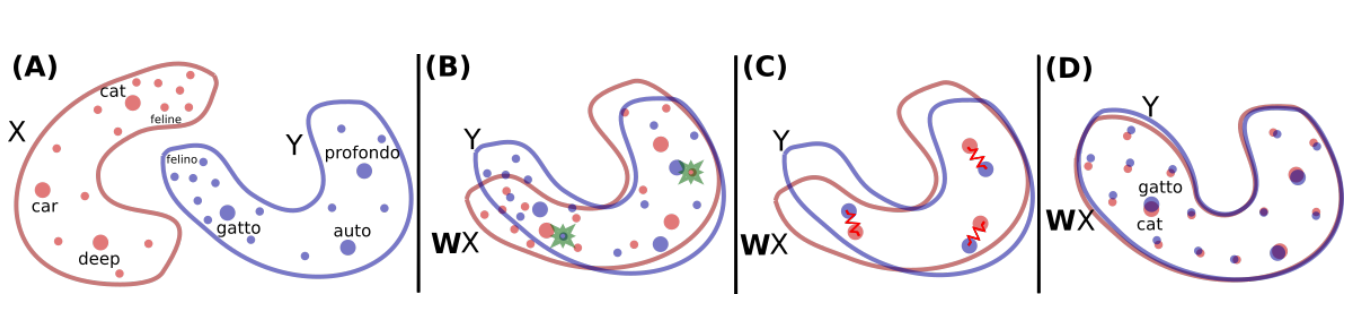
\includegraphics[width=1.0\linewidth, height=0.25\textheight]{figures/figure1.png}
\end{center}
(A) Two distributions of word embeddings are shown: \textbf{English words} in red, \(X\), and \textbf{Italian words} in blue, \(Y\), which we aim to \textbf{align}. Each dot represents a word, sized proportionally to its \textbf{frequency} in the training corpus. 

(B) Through \textbf{adversarial learning}, we learn a \textbf{rotation matrix} \(W\) that \textbf{aligns} the distributions. Green stars represent \textbf{randomly selected words} fed to the \textbf{discriminator}, which determines if the embeddings come from the same distribution. 

(C) The mapping \(W\) is \textbf{refined via Procrustes}, using \textbf{frequent words} from the previous alignment as \textbf{anchor points} to minimize an \textbf{energy function}, akin to a spring system. 

(D) \textbf{Translation} uses \(W\) and a \textbf{CSLS distance metric} that \textbf{expands dense areas} (e.g., around “cat”) to \textbf{reduce "hubness"}, making hubs like “cat” less close to other words compared to panel (A) (Figure 1, p. 3).

\normalsize
\end{block}

\begin{column}{\onecolwid}
	% Procrustes refinement
	\begin{block}{Refinement Procedure with Procrustes}
	    %\textbf{Refining the Mapping}
	    \begin{itemize}
	        \item \textbf{Initial mapping \( W \)} aligns well but \textbf{struggles with rare words}.
	        \item \textbf{Procrustes refinement} improves accuracy by enforcing \textbf{orthogonality}:
	        \longeqsize
	        \[
	            W^* = \argmin_{W \in O_d(\mathbb{R})} || W X - Y ||_F = UV^{T}, \quad \text{with } U,V^T\quad \text{from SVD}(YX^T) 
	        \]
	        \normalsize
	\item \textbf{Frequent words} as \textbf{anchors} build a high-quality dictionary.
	\item \textbf{Procrustes} is applied \textbf{iteratively} to refine \( W \).
	        %%O d ​ (R) represents the group of matrices that preserve lengths and angles (i.e., orthogonal transformations) in a �� d-dimensional space. The orthogonality constraint is used in Procrustes to ensure that the mapping �� W retains the geometric properties of the embedding spaces, such as angles and distances.
	    \end{itemize}
	\end{block}
\end{column}
\begin{column}{\onecolwid}
	%CSLS
	\begin{block}{Cross-Domain Similarity Local Scaling (CSLS)}
	    %\textbf{Improving Nearest Neighbor Matching}
	    \begin{itemize}
	        \item \textbf{CSLS reduces the effect of "hubs"} in dense areas, where some vectors are nearest neighbors for many others.
	\item \textbf{CSLS similarity measure}:
	\[
	    CSLS(W x_s, y_t) = 2 \cos(W x_s, y_t) - r_T(W x_s) - r_S(y_t)
	\]
	Where:
	\begin{align*}
	    r_T(W x_s) &= \frac{1}{K} \sum_{y_t \in N_T(W x_s)} \cos(W x_s, y_t), \\
	    r_S(y_t) &= \frac{1}{K} \sum_{x_s \in N_S(y_t)} \cos(x_s, y_t)
	\end{align*}
	\item \textbf{CSLS adjusts similarity based on word density, improving translation accuracy.}
	
	    \end{itemize}
	\end{block}
\end{column}


%Training and Architecture

\begin{block}{Training and Architectural Choices}
\begin{itemize}
    \item \textbf{Word Embeddings:} FastText embeddings with 300 dimensions, trained on Wikipedia; only the top 200k lowercased words.
    \item \textbf{Mapping \( W \):} A 300x300 matrix aligning source and target embeddings.
    \item \textbf{Discriminator:} MLP with two 2048-unit layers, Leaky-ReLU activation, 10\% dropout, and smoothing \( s = 0.2 \).
    \item \textbf{Training Procedure:} Discriminator is fed top 50,000 words only; orthogonal updates for stability.
    \item \textbf{Orthogonality Constraint:} Update rule \( W \leftarrow (1 + \beta)W - \beta(WW^{T})W \) with \( \beta = 0.01 \).
    \item \textbf{Dictionary Generation:} CSLS-selected mutual nearest neighbors boost translation accuracy.
    \item \textbf{Validation:} CSLS-based criterion, correlates with translation accuracy.
\end{itemize}
\end{block}


\end{column} 

\begin{column}{\sepwid}\end{column} 
\begin{column}{\onecolwid} 


\begin{block}{Results}
\begin{itemize}
\item \textbf{Procrustes - CSLS (supervised)}: Achieves \textbf{highest P@1 scores} across pairs, e.g., \textbf{81.4 (en-es)}, \textbf{82.9 (es-en)}, \textbf{72.4 (de-en)}. Outperforms other supervised methods like \textbf{Mikolov et al. (2013)} and \textbf{Smith et al. (2017)}.
\item \textbf{Adv - Refine - CSLS (unsupervised)}: Nearly matches \textbf{Procrustes - CSLS}, scoring \textbf{81.7 (en-es)}, \textbf{83.3 (es-en)}, and \textbf{74.0 (en-de)}. Often surpasses supervised methods.
\item \textbf{English-Esperanto BLEU Scores}: \textbf{Dictionary - NN}: 6.1 (en-eo), 11.9 (eo-en). \textbf{Dictionary - CSLS}: 11.1 (en-eo), 14.3 (eo-en), showing \textbf{improvement with CSLS}.
\item \textbf{Summary}: Both \textbf{Procrustes - CSLS} and \textbf{Adv - Refine - CSLS outperform} older methods; \textbf{Adv - Refine - CSLS} is highly competitive even without supervision.
\end{itemize}
\vspace{-1cm}
\normalsizecaption
\begin{table}[ht]
\centering
\setlength{\tabcolsep}{4pt}  % Reduce column padding
\renewcommand{\arraystretch}{0.9}
\resizebox{\columnwidth}{!}{ % Adjust the table to fit the column width
\begin{tabular}{|l|c|c|c|}
\hline
\textbf{Method} & \textbf{P@1} & \textbf{P@5} & \textbf{P@10} \\
\hline
\multicolumn{4}{|c|}{\textbf{Methods with cross-lingual supervision}} \\
\hline
Mikolov et al. (2013b)† & 10.5 & 18.7 & 22.8 \\
Dinu et al. (2015)† & 45.3 & 72.4 & 80.7 \\
Smith et al. (2017)† & 54.6 & 72.7 & 78.2 \\
Procrustes - NN & 42.6 & 54.7 & 59.0 \\
Procrustes - CSLS & \textbf{66.1} & 77.1 & 80.7 \\
\hline
\multicolumn{4}{|c|}{\textbf{Methods without cross-lingual supervision }} \\
\hline
Adv - CSLS & 42.5 & 57.6 & 63.6\\
Adv - Refine - CSLS & 65.9 & \textbf{79.7} & \textbf{83.1}\\
\hline
\end{tabular}
}
\end{table}
\vspace{-0.45cm}
\begin{table}[ht]
\centering
\setlength{\tabcolsep}{4pt}  % Reduce column padding
\renewcommand{\arraystretch}{0.9}
\resizebox{\columnwidth}{!}{ % Adjust the table to fit the column width
\begin{tabular}{|l|c|c|c|}
\hline
\textbf{Method} & \textbf{P@1} & \textbf{P@5} & \textbf{P@10} \\
\hline
\multicolumn{4}{|c|}{\textbf{Methods with cross-lingual supervision}} \\
\hline
Mikolov et al. (2013b)† & 12.0 & 22.1 & 26.7 \\
Dinu et al. (2015)† & 48.9 & 71.3 & 78.3 \\
Smith et al. (2017)† & 42.9 & 62.2 & 69.2 \\
Procrustes - NN & 53.5 & 65.5 & 69.5 \\
Procrustes - CSLS & \textbf{69.5} & \textbf{79.6} & \textbf{83.5} \\
\hline
\multicolumn{4}{|c|}{\textbf{Methods without cross-lingual supervision }} \\
\hline
Adv - CSLS & 47.0 & 62.1 & 67.8\\
Adv - Refine - CSLS & 69.0 & \textbf{79.7} & 83.1\\
\hline
\end{tabular}
}
\caption{English to Italian (1), Italian to English (2) word translation retrieval performance (P@1, P@5, P@10) for various methods with and without cross-lingual supervision, evaluated using P@k from 2,000 source queries and 200,000 target sentences. Embeddings from Smith et al. (2017). Results marked by † are theirs. Table 3, p. 8.}
\end{table}
\vspace{-2.7cm}

\end{block}
%----------------------------------------------------------------------------------------
%	REFERENCES
%----------------------------------------------------------------------------------------

\begin{block}{Reference}
\vspace{-0.78cm}
\begin{itemize}
\scriptsize
\setlength{\itemsep}{-2mm} 
\item Conneau, A., Lample, G., Ranzato, M. A., Denoyer, L., \& Jégou, H. (2018). Word translation without parallel data. arXiv. \url{https://doi.org/10.48550/arXiv.1710.04087}. Code implementation: \url{https://github.com/facebookresearch/MUSE}
\item Dinu, G., Lazaridou, A., \& Baroni, M. (2015). Improving zero-shot learning by mitigating the hubness problem. In \textit{Proceedings of the International Conference on Learning Representations, Workshop Track}.
\item Mikolov, T., Le, Q. V., \& Sutskever, I. (2013). Exploiting similarities among languages for machine translation. arXiv. \url{https://doi.org/10.48550/arXiv.1309.4168}.
\item Smith, S. L., Turban, D. H. P., Hamblin, S., \& Hammerla, N. Y. (2017). Offline bilingual word vectors, orthogonal transformations and the inverted softmax. In \textit{Proceedings of the International Conference on Learning Representations}.
\item Zhang, M., Liu, Y., Luan, H., \& Sun, M. (2017). Adversarial training for unsupervised bilingual lexicon induction. In \textit{Proceedings of the 53rd Annual Meeting of the Association for Computational Linguistics}.
\item Xing, C., Wang, D., Liu, C., \& Lin, Y. (2015). Normalized word embedding and orthogonal transform for bilingual word translation. In \textit{Proceedings of NAACL}.
\end{itemize}
\end{block}






\end{column}

\begin{column}{\sepwid}\end{column}

\end{columns}
\end{frame}
\end{document}